% !TeX spellcheck = en_US
%Aqui hay que mezclar sabiamente y en orden el paper de Viruses y los resultados del informe
\chapter{Model validation: The Australian case}\label{Australiano}

In this chapter we are going to check if we can obtain similar results to those in \cite{ali2013genital,fairley2009rapid} using the calibration parameters.

As we introduced in Chapter \ref{intro} \cite{ali2013genital}, there is a decrease on the number of infected persons and the number of persons with GW is already reported for Australia after two years of administering vaccinations to young girls. These results were more impressive than predicted by continuous models.

To check the reliability of the model, we simulated the HPV vaccination campaign carried out in Australia \cite{ali2013genital}, and compared them with the actual impact published \cite{ali2013genital}. In 2007, Australian health authorities started a vaccination program for 12--13 year-old girls with a~coverage of $73\%$ ($83\%$ in the first dose, $80\%$ in the second dose and $73\%$ in the third dose). In addition, from 2007 to 2009, there was a catch-up vaccination program for women aged 13--26 with a decreasing coverage with age until $52\%$ in women aged 20--26. The results can be summarized as follows \cite{ali2013genital}:

\begin{itemize}
	\item Two years after the vaccine was introduced, the proportion of genital warts diagnosed declined by a $59\%$ in vaccine eligible young women aged 12--26 years in $2007$, and by $39\%$ in men of the same age.
	\item No significant decline was observed in women or men older than $26$ years old, non-resident young women, or men who have sex with men (MSM).
\end{itemize}

Two different scenarios were considered to be simulated:

\begin{itemize}
	\item Scenario 1: vaccination of $83\%$ of the $14$ year-old girls (or younger girls) plus a catch-up with coverage $73\%$ for 14--26 year-old women.
	\item Scenario 2: vaccination of $73\%$ of $14$ year-old girls (or younger girls) plus a catch-up with a~vaccination coverage of $52\%$ for 14--26 year-old women.
\end{itemize}

These simulations represented the upper and lower bounds of the scenario implemented in Australia. 

\section{How to measure the decline}\label{sec:decline}%esto lo borré de otro capítulo y lo pongo ya aqui

We call $I$ the number of infected women of LR HPV 6 and/or 11 just before the starting of the vaccination campaign; we call $V = ( v_1, \ldots, v_N)$ to the number of infected women of LR HPV 6 and/or 11 every month from the starting of the vaccination program until the end of the simulation. Then,~the~vector 

\begin{equation}
100 \times \left( 1-\displaystyle\frac{v_1}{I}, \ldots, 1-\displaystyle\frac{v_N}{I} \right) \; 
\end{equation}

is a measure of the percentage of decline of the number of infected women of LR HPV 6 and/or 11 after the beginning of the vaccination campaign. This will also be applied to men and MSM.

In order to compare GW data given in \cite{ali2013genital} with our model, results referred to infected women of LR HPV 6 and/or 11, we should take into account that, whether a fixed proportion of HPV 6 and/or 11 infected individuals develops warts, the percentage of decline in warts and in infected women of LR HPV 6 and/or 11 will be comparable. 

Another important issue for the natural history of the disease is the persistence of the infection \cite{campos2014updated}. Our model does not consider the persistence ``a priori'', but we derive the cases of genital warts from the number of cases of infected individuals by taking this data into account.

\section{Does our model return similar values to those in \cite{ali2013genital}?}

In this section, we are going to show figures about prevalence and decline of the percentage of women, men and MSM infected of LR 6/11, the HPV type responsible of $90\%$ of genital warts. Taking into account that genital warts, in average, use to appear 6 months after the infection, the figures about prevalence or decline will be a good estimation of the prevalence and the  decline of genital warts.  

Figure \ref{fig:prev_AUS_6_11} shows the percentage of women, men and MSM aged 14-26 infected of LR 6/11 after starting the vaccination program in both simulated scenarios. We can see the fast decrease for women and men in both scenarios from the very beginning. MSM remain constant. 

\begin{figure}[!]
	\centering
	\begin{tabular}{cc}
		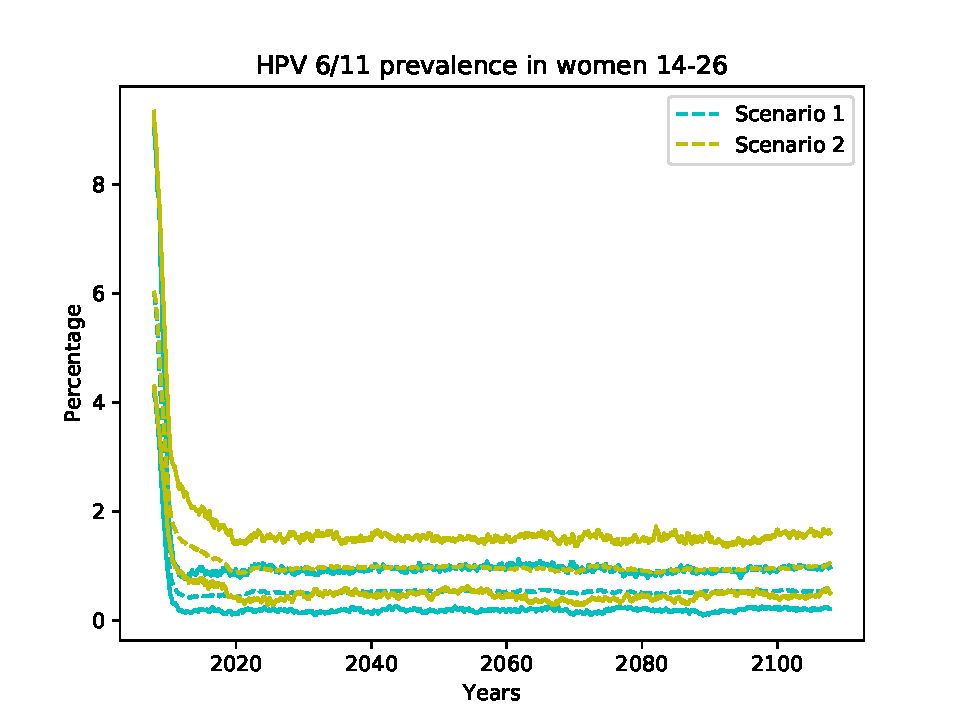
\includegraphics[width=0.5\linewidth]{IMGs/3.-Australia/retrieve_14_26_verr_muj.pdf}	& 
		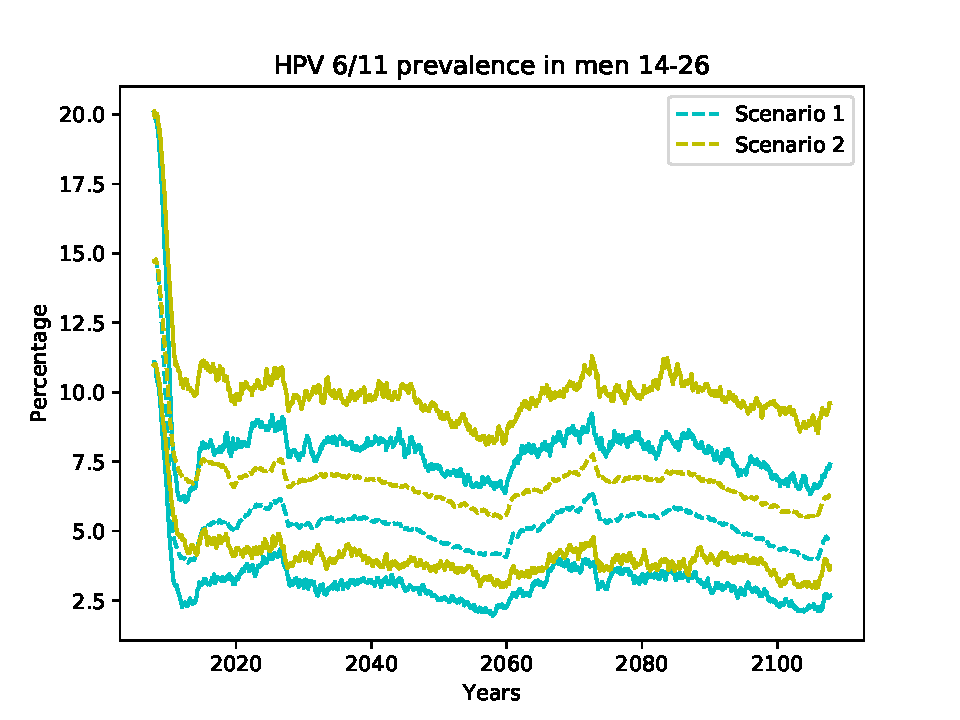
\includegraphics[width=0.5\linewidth]{IMGs/3.-Australia/retrieve_14_26_verr_hom.pdf}  \\ 
		(a)	& (b) \\ 
		\multicolumn{2}{c}{ 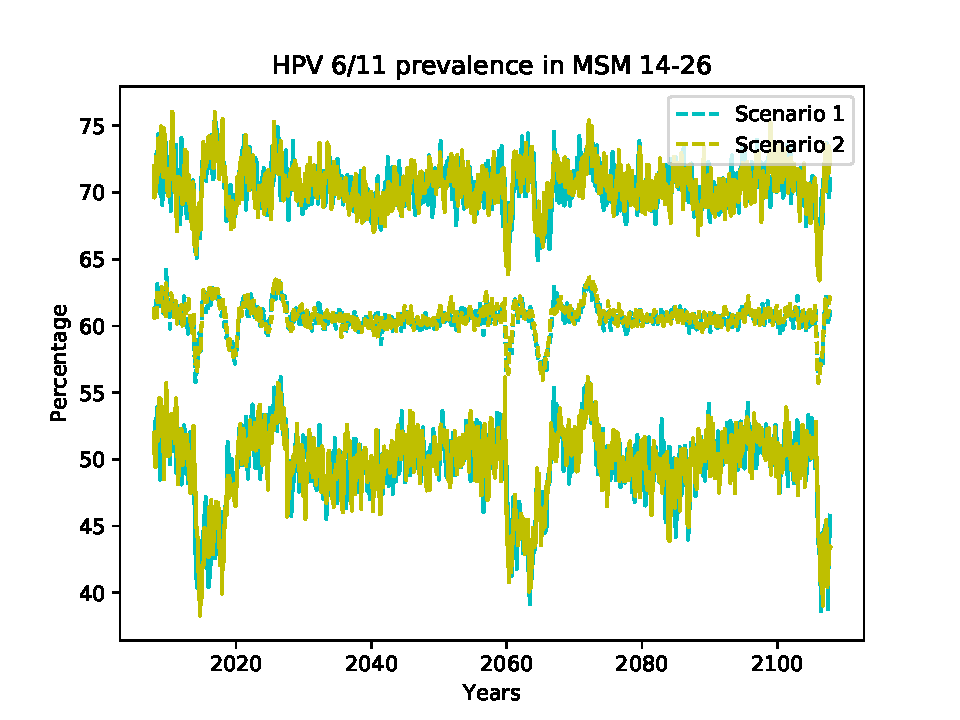
\includegraphics[width=0.5\linewidth]{IMGs/3.-Australia/retrieve_14_26_verr_MSM.pdf} } \\ 
		\multicolumn{2}{c}{(c)} \\ 
	\end{tabular} 
	\caption{Percentage of women (a), men (b) and MSM (c) aged 14-26 infected of LR HPV 6 and/or 11 after the implementation of the vaccination program. The cyan lines correspond to the average and $95\%$ confidence interval for Scenario 1 and the yellow lines to Scenario 2.  We can see the fast decrease for women and men in both scenarios from the very beginning. However, there is not effect on MSM.}
	\label{fig:prev_AUS_6_11}	
\end{figure}

In Figure \ref{fig:decline_AUS_6_11}, we have plotted the same data as in Figure \ref{fig:prev_AUS_6_11} but from another point of view: the average percentage of decline of women and men infected of LR HPV 6 and/or 11. As the vaccination program progresses over time, the percentage of decline obviously grows. After 2 years, the model shows a decline of

\begin{itemize}
	\item Scenario 1: $72.0\%$ with CI $95\%$ $[67.7\%, 76.5\%]$ for women and $38.9\%$ with CI $95\%$ $[32.0\%, 45.5\%]$ for men. 
	\item Scenario 2: $54.8\%$ with CI $95\%$ $[48.5\%, 59.0\%]$ for women and $27.7\%$ with CI $95\%$ $[21.3\%, 34.5\%]$ for men. 
\end{itemize}

Australian reported levels of decline ($59\%$ in women and $39\%$ in men aged 14-26) will be reached by the model after

\begin{itemize}
	\item Scenario 1: $1.66$ years with CI $95\%$ $[1.5, 1.75]$ for women and $2.0$ years with CI $95\%$ $[1.75, 2.16]$ for men,
	\item Scenario 2: $2.1$ years with CI $95\%$ $[2.0, 2.33]$ for women and $2.42$ years with CI $95\%$ $[2.08, 2.83]$ for men.
\end{itemize}

\begin{figure}[!]
	\centering
	\begin{tabular}{cc}
		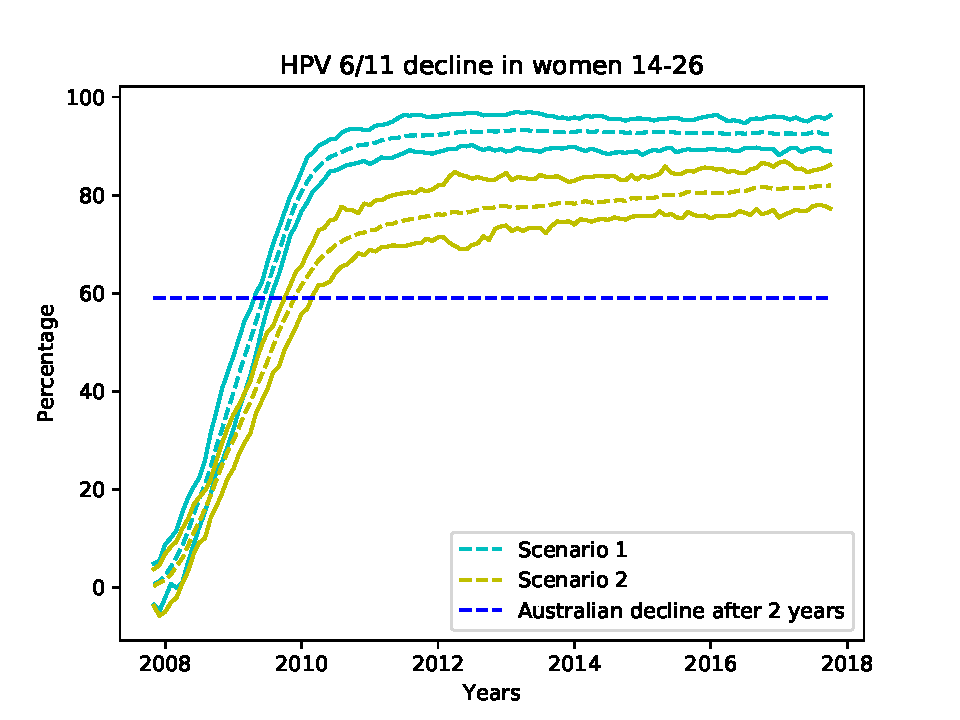
\includegraphics[width=0.45\linewidth]{IMGs/3.-Australia/decline_14_26_verr_muj.pdf}	& 
		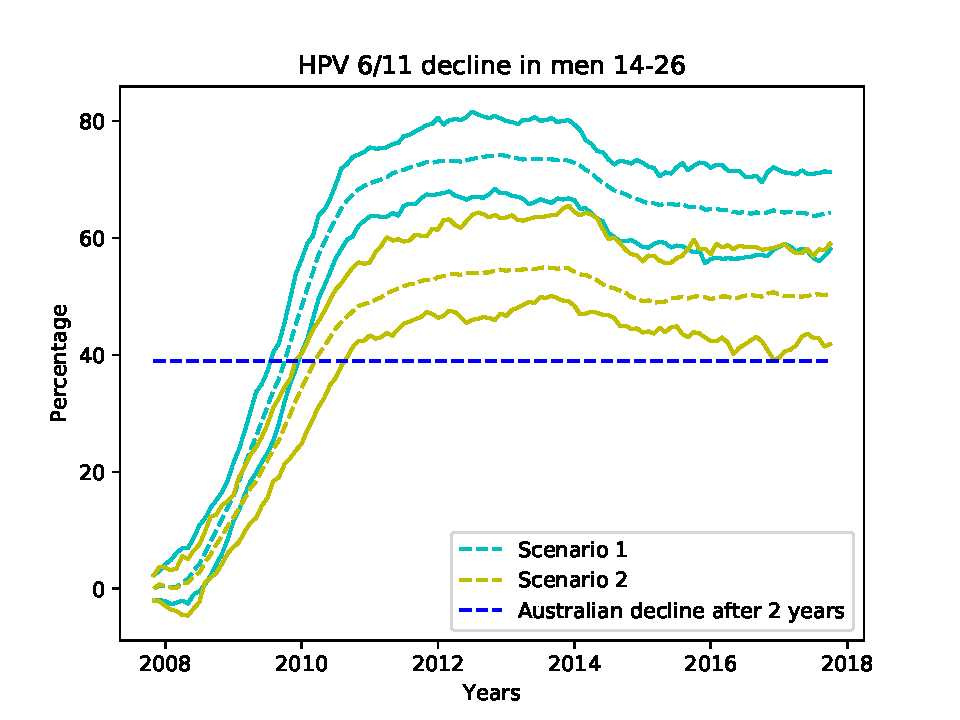
\includegraphics[width=0.45\linewidth]{IMGs/3.-Australia/decline_14_26_verr_hom.pdf}  \\ 
		(a)	& (b) 
	\end{tabular} 
	\caption{Percentage of decline of women (a) and men (b) aged 14-26 infected of LR HPV 6 and/or 11 (and consequently of genital warts) after the implementation of the vaccination program. The cyan lines correspond to the average and $95\%$ confidence interval for Scenario 1 and the yellow lines to Scenario 2. After 2 years, the model shows a decline of $72\%$ for Scenario 1 and $54.8\%$ for Scenario 2, in average, for women and $38.9\%$ for Scenario 1 and $27.7\%$ for Scenario 2, in average, for men.}
	\label{fig:decline_AUS_6_11}
\end{figure}

No significant impact on the rate of infection was observed in men aged 27-64, 2 years after the implementation of the vaccination program (Figure \ref{fig:decline_AUS_6_11_27_64}) and the same in women and MSM agreeing the observations reported in \cite{ali2013genital}. It can be explained by the fact that, usually, individuals have sexual intercourses with people more or less the same age. 

Then, our model predicts figures close to the ones given in \cite{ali2013genital}.

\begin{figure}[!]
	\centering
	\begin{tabular}{cc}
		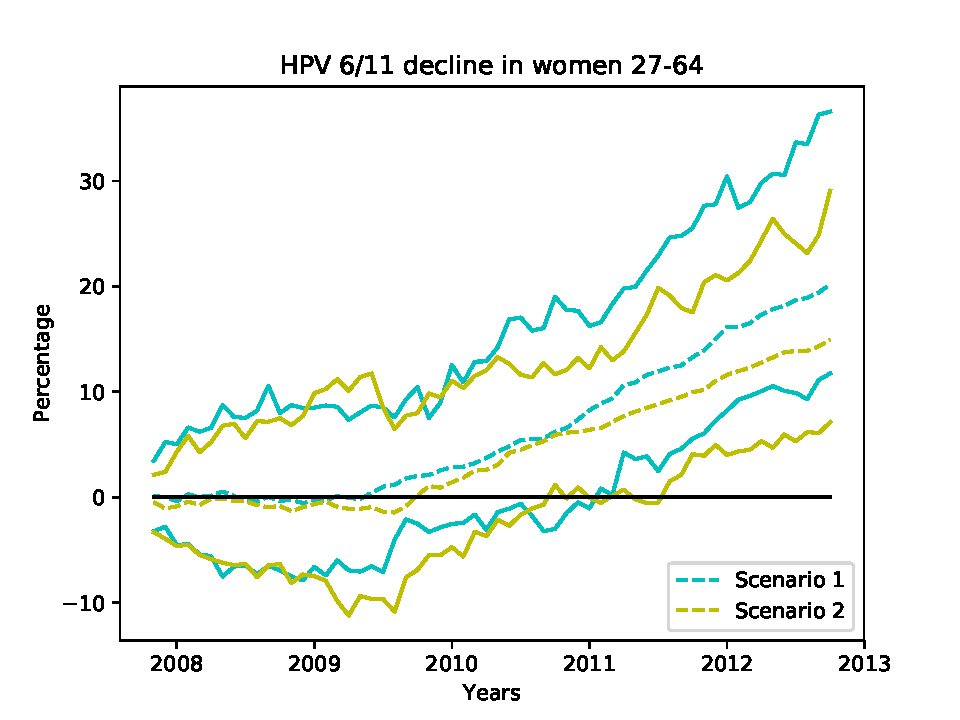
\includegraphics[width=0.5\linewidth]{IMGs/3.-Australia/decline_27_64_verr_muj.pdf}	& 
		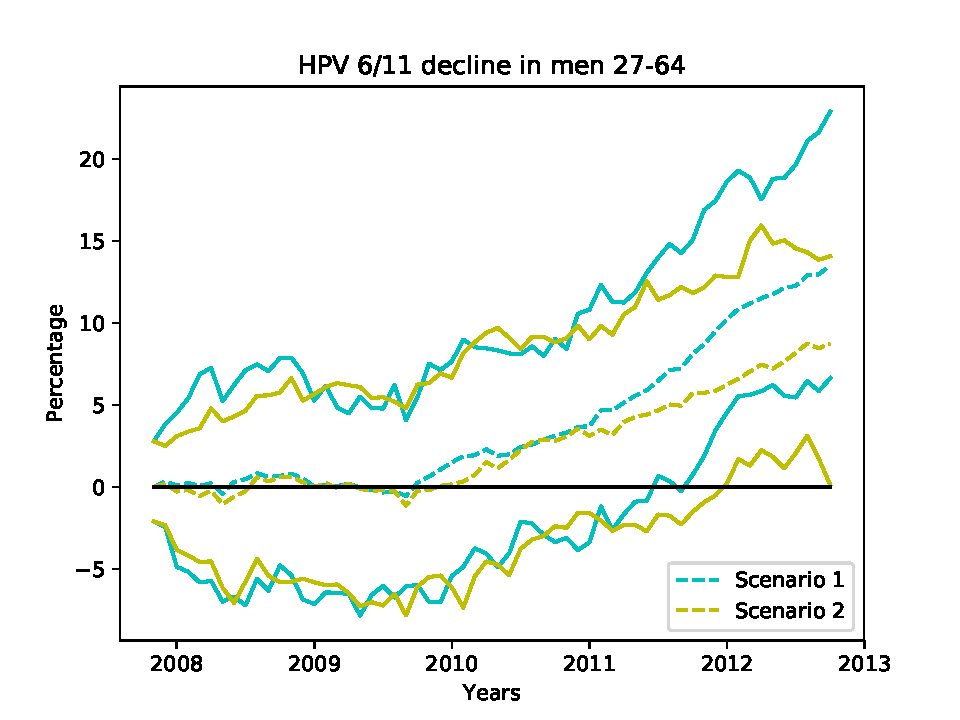
\includegraphics[width=0.5\linewidth]{IMGs/3.-Australia/decline_27_64_verr_hom.pdf}  \\ 
		(a)	& (b) \\ 
		\multicolumn{2}{c}{ 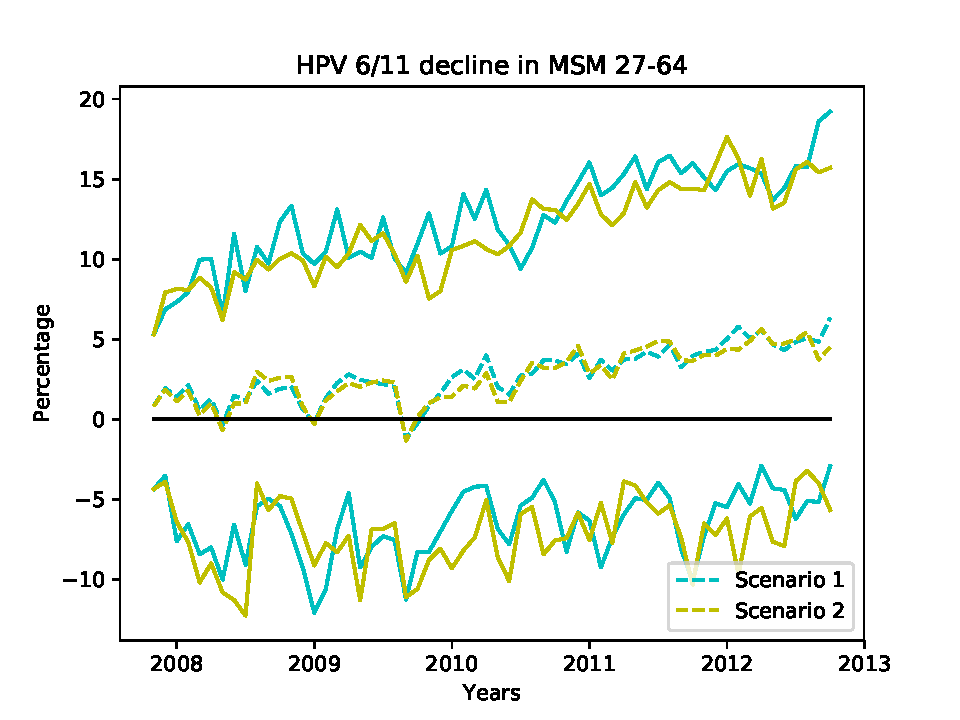
\includegraphics[width=0.5\linewidth]{IMGs/3.-Australia/decline_27_64_verr_MSM.pdf} } \\ 
		\multicolumn{2}{c}{(c)} \\ 
	\end{tabular} 
	\caption{Percentage of decline of women (a), men (b) and (c) MSM aged 27-64 infected of LR HPV 6 and/or 11 (and consequently of genital warts) after the implementation of the vaccination program in both scenarios. The cyan lines correspond to the average and $95\%$ confidence interval for Scenario 1 and the yellow lines to Scenario 2. Notice that, in average, no significant decline appears in the 5 years after the implementation of the vaccination program.}
\label{fig:decline_AUS_6_11_27_64}
\end{figure}

\section{Study of the herd immunity effect over HPV LR infection}
The herd immunity effect in both scenarios is shown in Figure \ref{fig:decline_AUS_6_11_14_64} for women, men and MSM. Notice that, in men and MSM, any decline is due to herd immunity. The decline in the whole female population appears when the lines representing their decline are over the vaccination lines (blue for Scenario 1 and green for Scenario 2) also shown in this figure. The herd immunity effect starts after 

\begin{itemize}
	\item for women
	\begin{itemize}
		\item Scenario 1: $0.58$ years with CI95\% $[0.0, 22.1]$.
		\item Scenario 2: $0.58$ years with CI95\% $[0.0, 22.1]$.
	\end{itemize}
	\item for men
	\begin{itemize}
		\item Scenario 1: $0.0$ years with CI95\% $[0.0,0.83]$.
		\item Scenario 2: $0.0$ years with CI95\% $[0.0,0.83]$.	
	\end{itemize}
\end{itemize}

The herd immunity effect starts very quickly for men. For MSM, there is not a clear herd immunity effect because the decline is stable over the time. For women, we can see that, practically, the CI$95\%$ decline lines are over the vaccination lines in both scenarios. This means that, in the worst case, only the vaccinated women will be protected and in the best case, almost all women will be protected by vaccination or by herd immunity effect.

\begin{figure}[!]
	\centering
	\begin{tabular}{cc}
		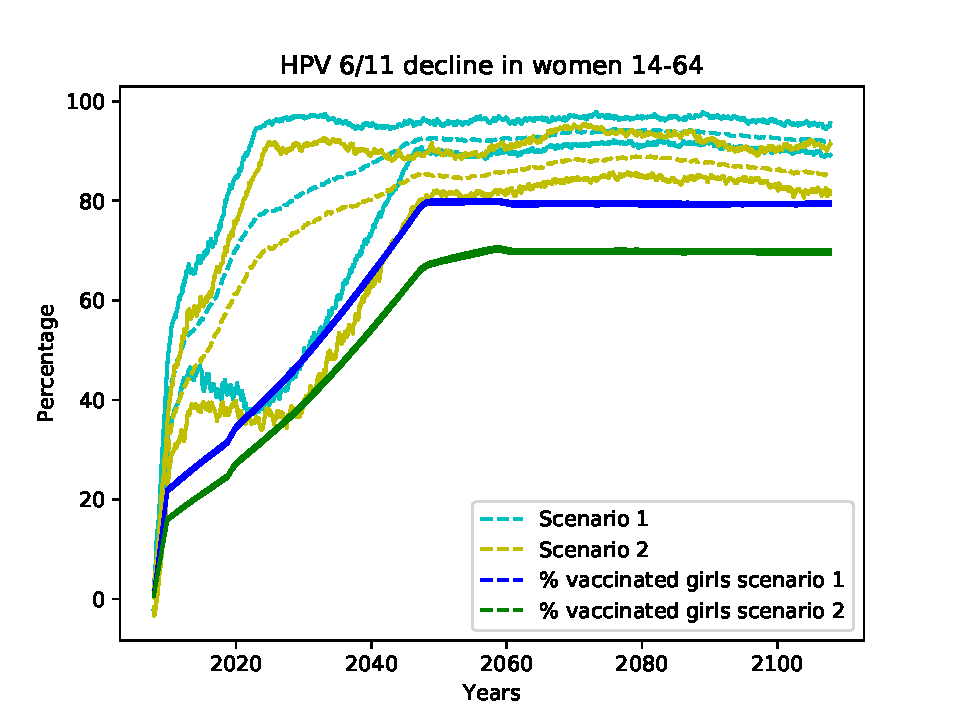
\includegraphics[width=0.45\linewidth]{IMGs/3.-Australia/decline_14_64_verr_muj.pdf}	& 
		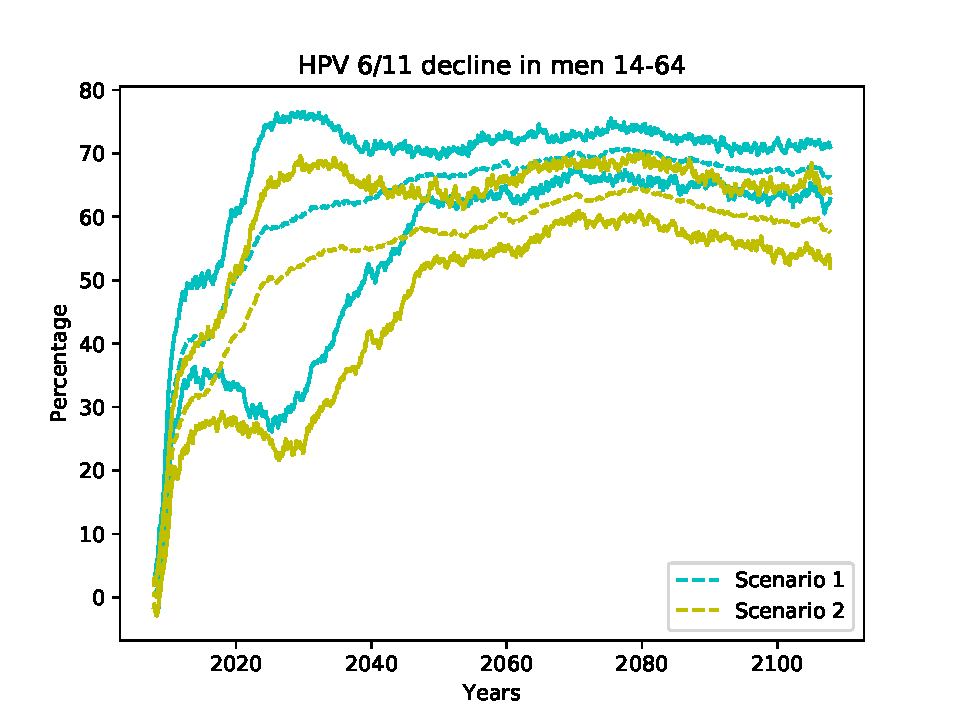
\includegraphics[width=0.45\linewidth]{IMGs/3.-Australia/decline_14_64_verr_hom.pdf}  \\ 
		(a)	& (b) \\ 
		\multicolumn{2}{c}{ 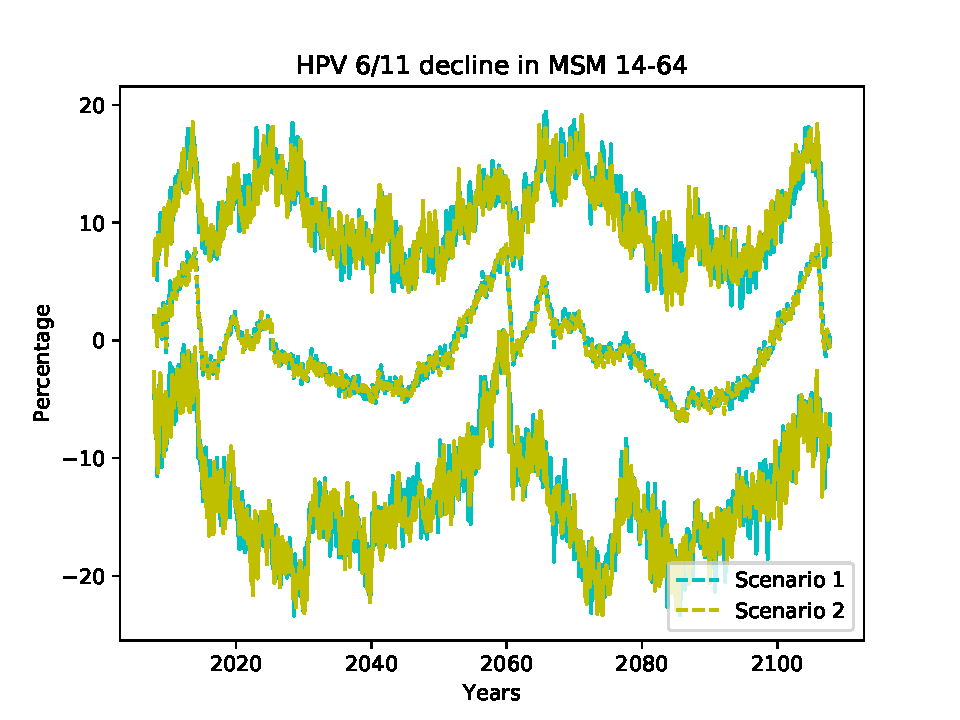
\includegraphics[width=0.5\linewidth]{IMGs/3.-Australia/decline_14_64_verr_MSM.pdf} } \\ 
		\multicolumn{2}{c}{(c)} \\ 
	\end{tabular} 
	\caption{Percentage of decline of women (a), men (b) and MSM (c) aged 14-64 for the vaccination program in Australia. The cyan lines correspond to the average and $95\%$ confidence interval for Scenario 1 and the yellow lines to Scenario 2. In the figure (a), blue and green lines correspond to women vaccination percentage for Scenario 1 and 2, respectively. Notice that the herd immunity effect contributes to the decline in the number of infections in men and the decline in the number of infections for unvaccinated women. This latter can be seen when the decline lines are over the vaccination line. However, any herd immunity effect can be seen in MSM.}
	\label{fig:decline_AUS_6_11_14_64}
\end{figure}

Notice that the herd immunity effect is very clear within the CI$95\%$ both for women and men, but it does not appear in the MSM population. In the best case scenario, the MSM subpopulation achieves a constant protection level of $10\%-15\%$. This could be attributed to the way in which the MSM individuals are connected: with a very large number of LSPs among them and some casual links with women with large LSPs.

\section{Effect of the reduction of the vaccine effectiveness in the catch-up vaccination}\label{sec:australia_sfuka}
In the reference \cite{Skufca}, the authors perform a literature review where they show that the effectiveness of the HPV vaccine on cervical abnormalities is between $20\%-54\%$ instead of the assumed $96.5\%$. This means that the vaccine effectiveness experiments a reduction in those women who had previous contact with the virus.

To study the effect of this catch-up loss of the effectiveness, we propose the simulation of the following two scenarios: 

\begin{itemize}
	\item Scenario 1: vaccination of $83\%$ of the $14$ year-old girls (or younger girls) plus a catch-up with coverage $73\%$ for 14--26 year-old women with $54\%$ of catch-up effectiveness.
	\item Scenario 2: vaccination of $73\%$ of $14$ year-old girls (or younger girls) plus a catch-up with a~vaccination coverage of $52\%$ for 14--26 year-old women with $20\%$ of catch-up effectiveness.
\end{itemize}

The above scenarios consist of a variation of the scenarios already proposed  for Australia at the beginning of this chapter, but now, considering the reduction of the effectiveness in the catch-up vaccination. The simulations consider upper and lower scenarios. 

In the following, we present the compared results with the scenarios without loss of effectiveness in the catch-up vaccination. Then, after 2 years, the model declines are

\begin{itemize}
	\item Ali et al. \cite{ali2013genital}: $59\%$ for women and $39\%$ for men.
	\item Catch-up without loss of effectiveness:
	\begin{itemize}
	\item Scenario 1: $72.0\%$ with IC $95\%$ $[67.7\%, 76.5\%]$ for women and $38.9\%$ with IC $95\%$ $[32.0\%, 45.5\%]$ for men. 
	\item Scenario 2: $54.8\%$ with IC $95\%$ $[48.5\%, 59.0\%]$ for women and $27.7\%$ with IC $95\%$ $[21.3\%, 34.5\%]$ for men.
	\end{itemize} 
   	\item Catch-up with loss of effectiveness:
    	\begin{itemize}
    	\item Scenario 1: $45.68\%$ with IC $95\%$ $[40\%, 51.9\%]$ for women and $23.2\%$ IC $95\%$ $[18\%, 32.5\%]$ for men.
    	\item Scenario 2: $17.5\%$ IC $95\%$ $[11\%, 25.4\%]$ for women and $9\%$ IC $95\%$ $[4.7\%, 13\% ]$ for men.
    \end{itemize} 
\end{itemize}

The levels of decline reported in \cite{ali2013genital}, that is $59\%$ in women and $39\%$ in men aged 14-26, will be reached after

\begin{itemize}
	\item Ali et al. \cite{ali2013genital}: 2 years
	\item Catch-up without loss of effectiveness:
	\begin{itemize}
	\item Scenario 1: $1.66$ years with CI $95\%$ $[1.5, 1.75]$ for women and $2.0$ years with CI $95\%$ $[1.75, 2.16]$ for men,
	\item Scenario 2: $2.1$ years with CI $95\%$ $[2.0, 2.33]$ for women and $2.42$ years with CI $95\%$ $[2.08, 2.83]$ for men.
	\end{itemize}
	\item Catch-up with loss of effectiveness:
	\begin{itemize}
	\item Scenario 1: $2.75$ years with CI $95\%$ $[2.25, 4]$ for women and $2.9$ years with CI $95\%$ $[2.4, 4.6]$ for men,
	\item Scenario 2: $8.41$ years with CI $95\%$ $[6.7, 9.3]$ for women and $10$ years with CI $95\%$ $[6, 11.2]$ for men.
	\end{itemize} 
\end{itemize}

The differences among the obtained results seem to point out that the catch-up effectiveness for genital warts may be higher than the figures collected in \cite{Skufca} for cervical abnormalities.  

\section{Discussion}
The random network of sexually transmitted HPV including up to $100,000$ nodes, was developed to fit the data of surveys concerning the number of sexual partners throughout life. Standard continuous models are insufficient to accurately predict transmission because they do not account for the individual to individual transmission of the infection, the role of hubs in disseminating the virus through the rest of the population and neither the vaccination campaigns targeting specific groups of individuals.

This network has successfully been applied to the stable state of infections by LR and HR HPV genotypes in Spain  \cite{Acedo2017}. In this study we mimicked the results found in the HPV vaccination campaign in Australia \cite{ali2013genital}, and showed very reliable results. 

Models based upon continuous differential equations predict a slower decrease in the number of infected individuals after implementing similar vaccination campaigns \cite{elbasha2007model}. Hence, the case of the HPV vaccination in Australia provides one of the best real scenarios for testing new network models in mathematical epidemiology. There is an on-going debate on the pertinence of an approach based upon networks on epidemiology \cite{Eubank} and this work contributes to show the necessity of such an approach in many cases, in particular, in those corresponding to STD.

To validate the model, we used the Australian experience, with two different vaccination coverages: routinely vaccination campaign for $12-13$ year-old girls with a coverage of $73\%$ and $83\%$ and a catch-up program in the $14-26$ age group with an average coverage of $52\%$ and $73\%$. This program revealed an important herd immunity effect \cite{ali2013genital}, so that vaccination decreased the incidence of genital warts (GW) even in the non-vaccinated men because of the protection of infection conferred by the vaccine, and the decreased transmission of the virus.

The model predicted a fast decline in the number of infections parallel to the decline in the number of GW in Australia with very similar values. However, this model was built with Spanish data on sexual behavior \cite{INE} and prevalence of HPV infection \cite{castellsague2012prevalence}, that might differ from the Australian one, and may explain the minor differences found between the model and the actual data published. Herd immunity in this model of STD is predicted much sooner than in other highly transmitted aerial transported infectious diseases as influenza or RSV, due to the structure of the network. This supports the need to build appropriate LSP networks. 

Also, we performed simulations taking into account the loss of effectiveness in the catch-up vaccination following the figures collected in \cite{Skufca}. The results of decline were compared with the previous simulations for Australia and those presented in \cite{ali2013genital}. It seems that the catch-up effectiveness for genital warts may be higher than the figures collected in \cite{Skufca} for cervical abnormalities.  

Other models have also predicted the protection of males by vaccinating girls and women, but only for men, as the model used by Bogaards et al. \cite{bogaards2015direct}. This model uses Bayesian techniques to study the herd immunity effect. However, in contrast with our model, it does not take into account the dynamics of the HPV transmission, the importance of age-groups and the different roles they play in the propagation of these viruses or the links among the MSM subpopulation and the heterosexual network. In this sense, a network model is required to study the impact of the vaccination strategies in short, medium and long time scales.

Vaccination strategies should seek an optimal effectiveness and efficiency. In this case, it can be seen the quick apparition of the herd immunity effect on males and females only vaccinating women. However, the herd immunity effect does not appear in  MSM. This can be the consequence of the large LSP numbers for MSM and their casual connections with women with large LSP numbers in the heterosexual subnetwork.

The model considers a quiet close community, where there is not much contact with other communities. This may not be the case in Spain which in $2016$ received over $75$ million tourists \cite{INEturismo}, representing almost the double of the number of Spanish inhabitants, and where sexual contacts are frequent. This may bias the results, as the herd immunity in Spain may not be so clear as in countries with less tourism. Nevertheless we will study the effect of tourism in Spain.

Another issue that we must take into account, is the modelling of the population with a high number of contacts because these individuals are hubs in the network whose vaccination may induce a faster decline of the virus prevalence. Our approach is rather conservative in the assignment of LSP for men and women with $10$ or more links because we assume that all of them have similar LSP. However, it is expected that individuals with extreme values of LSP are favouring the transmission of HPV in such a way that  a targeted vaccination can show its benefit in a very short time.
